\section{Auswertung}
\label{sec:Auswertung}
\subsection{Darstellung der aufgenommenen Messwerte und verwendete Herstellerangaben}
\label{subsec:erdbfeld}
In den Tabellen \ref{tab:Messwerte1} und \ref{tab:Messwerte2} sind die aufgenommenen Stromstärken für Horizontal- und Sweepfeld im Resonanzfall zu den unteschiedlichen Frequenzen des Hochfrequenzfeldes aufgetragen.
\begin{table}[H]
  \centering
  \caption{Erste Messung: Im Resonanzfall gemessene Stromstärken an Sweep-(S) und Horizontalfeldspule(H) bei unterschiedlichen Frequenzen des RF-Feldes für beide Rubidium Isotope (A,B).}
  \label{tab:Messwerte1}
  \begin{tabular}{c|cc|cc}
  & Sweepfeld & & Horizontalfeld &\\
  \hline
  $\nu_1$ in kHz& $I_{S,A}$ in $\si{\milli\ampere}$& $I_{S,B}$ in \si{\milli\ampere}&$I_{H,A}$ in \si{\milli\ampere}& $I_{H,B}$in \si{\milli\ampere}\\
  \hline
  98  &446 &564 &0   &0   \\
  194 &681 &910 &0   &0   \\
  296 &472 &828 &24  &24  \\
  393 &353 &818 &42  &42  \\
  499 &274 &863 &66  &66  \\
  608 &141 &862 &90  &90  \\
  706 &064 &900 &114 &114 \\
  802 &602 &837 &90  &138 \\
  916 &735 &414 &102 &198 \\
  1016&787 &428 &114 &222 \\
  \hline
  \end{tabular}
\end{table}
\begin{table}[H]
  \centering
  \caption{Zweite Messung: Im Resonanzfall gemessene Stromstärken an Sweep-(S) und Horizontalfeldspule(H) bei unterschiedlichen Frequenzen des RF-Feldes für beide Rubidium Isotope (A,B).}
  \label{tab:Messwerte2}
  \begin{tabular}{c|cc|cc}
  & Sweepfeld & & Horizontalfeld &\\
  \hline
  $\nu_2$ in kHz& $I_{S,A}$ in $\si{\milli\ampere}$& $I_{S,B}$ in \si{\milli\ampere}&$I_{H,A}$ in \si{\milli\ampere}& $I_{H,B}$in \si{\milli\ampere}\\
  \hline
  109 &630 &760  &0   &0   \\
  210 &619 &856  &-6  &-6  \\
  303 &578 &933 &12  &12  \\
  400 &454 &927 &36  &36  \\
  507 &240 &841  &66  &66  \\
  613 &151 &876  &90  &90  \\
  707 &379 &940 &90  &108 \\
  805 &166 &542  &120 &162 \\
  901 &695 &766  &102 &168 \\
  1027&883 &453  &114 &222 \\
  \hline
  \end{tabular}
\end{table}
 Um die Stromstärkenin magnetische Feldstärken umzurechnen wird die Formel
\begin{equation}
  B = \mu_0\frac{ I \cdot N}{\sqrt{125}\cdot R}
  \label{eqn:Spulenbfeld}
\end{equation}
verwendet. Die Windungszahlen N und der Radius R der verschiedenen Spulen werden der Anleitung\cite{Anleitung} entnommen und sind in Tabelle \ref{tab:Spulendaten} aufgeführt.
\begin{table}[H]
  \centering
  \caption{Herstellerangaben für Windungszahl $N$ und Radius $r$ der drei Verwendeten Spulenpaare}
  \label{tab:Spulendaten}
  \begin{tabular}{c|c|c}
    Spule & $N$ &$R$ in cm\\
    \hline
    Horizontalfeld& 151 & 15.79\\
    Vertikalfeld  & 20  & 11.735\\
    Sweep-Feld    & 11  & 16.39\\
  \end{tabular}
\end{table}
\subsection{Berechnung der Verschiebung des Gesamthorizontalfeldes durch das Edrmagnetfeld}
\label{erdfeld}
Aus den Angaben für die Vertikalfeldspule berechnet sich nach \eqref{eqn:Spulenbfeld} ein vertikales Erdmagnetfeld der Feldstärke $B_v = \SI{49.19}{\micro\tesla}$. Die magnetischen Feldstärken von Sweep- und Horizontalfeld werden nun einzeln für jede Frequenz addiert. Das Gesamthorizontalfeld wird dann daraus, ebenfalls mithilfe von Formel \eqref{eqn:Spulenbfeld}, berechnet.
Die ermittelten Werte sind für beide Messreihen in Abhängigkeit von den jeweiligen Frequenzen $\nu_1$ und $\nu_2$ in den Tabellen \ref{tab:gesamt1} und  \ref{tab:gesamt2} dargestellt.
\begin{table}[H]
  \centering
  \caption{Messung 1: Summe aus Sweep- und Horizontalfeld zur jeweiligen Frequenz des Hochfrequenzfeldes für beide Isotope (A,B).}
  \label{tab:gesamt1}
\begin{tabular}{c||c|c|c}
$\nu_1$ in $\si{\kilo\hertz}$& $\symup{B_{1A}}$ in $\si{\micro\tesla}$&$\symup{B_{1B}}$ in $\si{\micro\tesla}$\\
\hline
98  & 26.9 & 34.1  & \\
194 & 41.1 & 54.9  & \\
296 & 49.5 & 71.0  & \\
393 & 58.1 & 86.2  & \\
499 & 74.4 & 110.0 & \\
608 & 87.4 & 130.9 & \\
706 & 103.8& 154.3 & \\
802 & 115.3& 171.5 & \\
916 & 133.8& 198.6 & \\
1016& 147.5& 220.5 & \\
\end{tabular}
\end{table}
\begin{table}[H]
  \centering
  \caption{Messung 2: Summe aus Sweep- und Horizontalfeld zur jeweiligen Frequenz des Hochfrequenzfeldes für beide Isotope (A,B).}
  \label{tab:gesamt2}
\begin{tabular}{c||c|c|c}
$\nu_2$ in $\si{\kilo\hertz}$& $\symup{B_{2A}}$ in $\si{\micro\tesla}$&$\symup{B_{2B}}$ in $\si{\micro\tesla}$\\
\hline
109 & 38.0 & 45.9 &\\
210 & 32.1 & 46.4 &\\
303 & 4.54 & 66.8 &\\
400 & 59.0 & 87.5 &\\
507 & 72.4 & 108.6&\\
613 & 88.0 & 131.8&\\
707 & 101.8& 151.4&\\
805 & 115.3& 174.8&\\
901 & 131.4& 193.6&\\
1027& 153.3& 222.0&\\
\end{tabular}
\end{table}
Um die Verschiebung des Feldes durch das horizontale Erdmagnetfeld zu bestimmen, wird an den obigen Daten eine lineare Regression an der Funktion
\begin{equation*}
  b(\nu) = m\cdot\nu + B_{hor}
\end{equation*}
durchgeführt.
Der y-Achsenabschnitt $B_{hor}$ der Ausgleichsgraden entspricht dann der horizontalen Komponente des Erdmagnetfeldes.
Die Ausgleichsrechnungen für beide Messungen sind in den Abbildungen \ref{fig:Bfeldfit1} und \ref{fig:Bfeldfit2} dargestellt.

\begin{figure}[H]
  \centering
  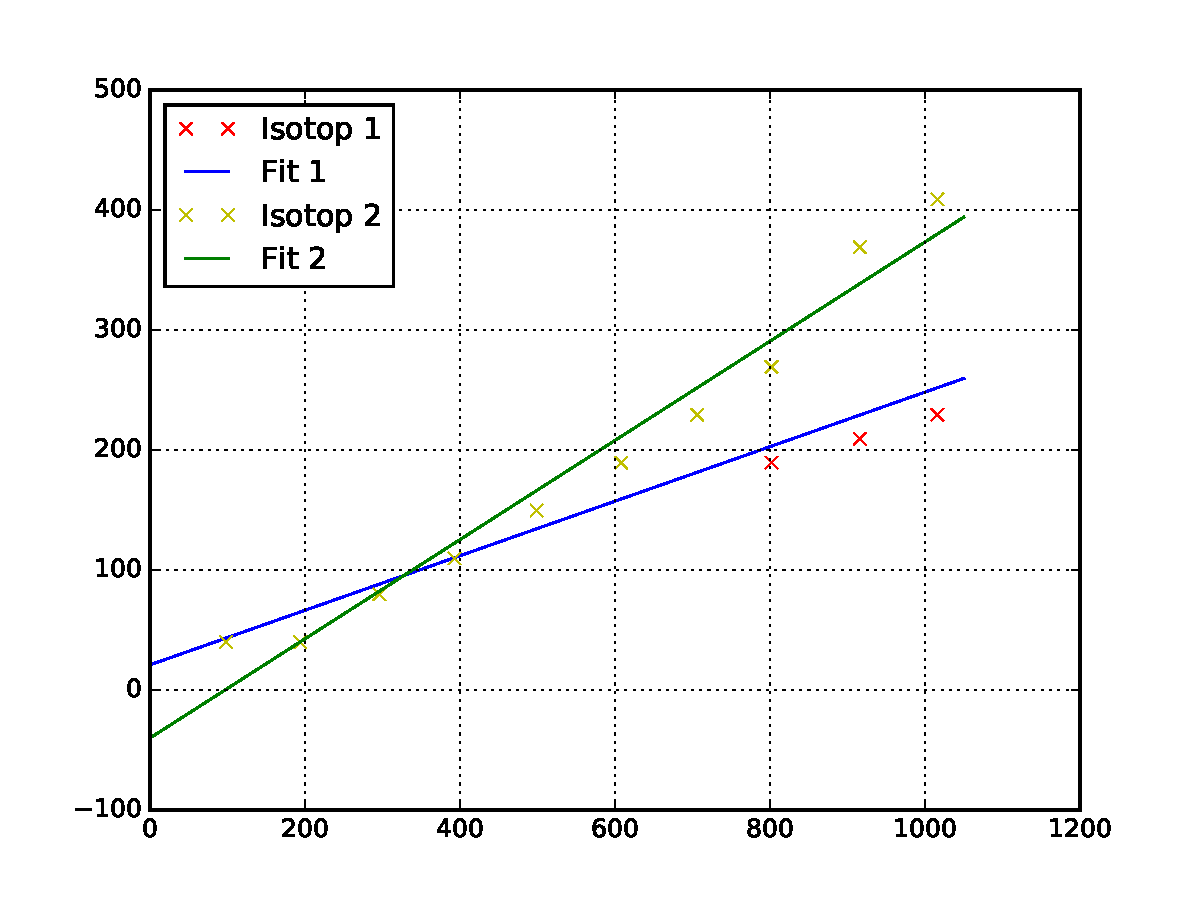
\includegraphics[width=\textwidth]{plots/Bfeldfit1}
  \caption{Linearer Fit der Messwerte der ersten Messung für Frequenz und horizontales Magnetfeld beider Isotope zur Bestimmung der Horizontalkomponente des Erdmagnetfeldes.}
  \label{fig:Bfeldfit1}
\end{figure}
\begin{figure}[H]
  \centering
  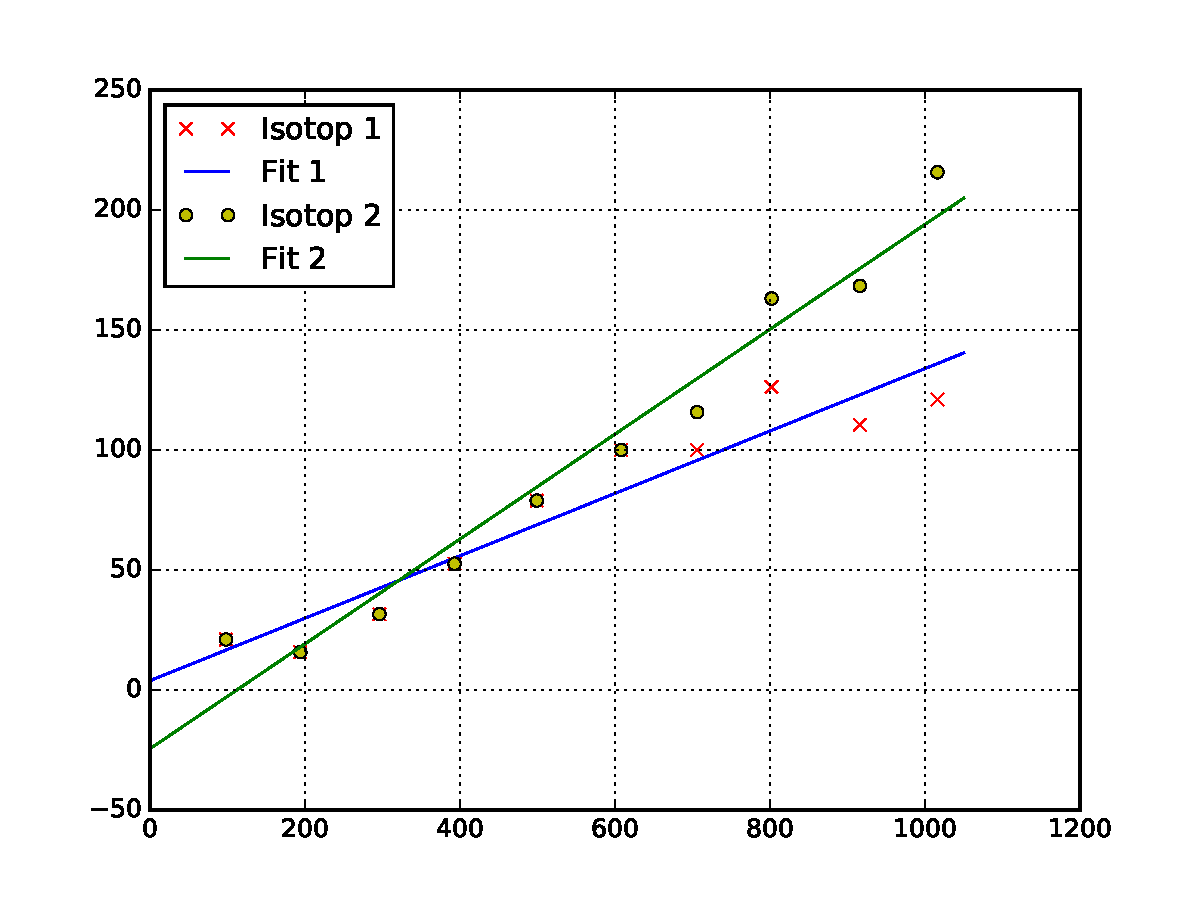
\includegraphics[width=\textwidth]{plots/Bfeldfit2}
  \caption{Linearer Fit der Messwerte der zweiten Messung für Frequenz und horizontales Magnetfeld beider Isotope zur Bestimmung der Horizontalkomponente des Erdmagnetfeldes.}
  \label{fig:Bfeldfit2}
\end{figure}
Die errechneten Fitparameter lauten:
\begin{center}
  $m_{1A} =\SI{0.131 \pm 0.003}{\micro\tesla\per\kilo\hertz}$ \,\,$b_{1A} =\SI{11.3 \pm 2.1}{\micro\tesla}$\\
  $m_{1B}=\SI{0.202 \pm 0.004}{\micro\tesla\per\kilo\hertz}$ \,\,$b_{1B} =\SI{11.5 \pm 2.2}{\micro\tesla}$\\
  $m_{2A} =\SI{0.134 \pm 0.007}{\micro\tesla\per\kilo\hertz}$ \,\,$b_{2A} =\SI{8.87 \pm 4.5}{\micro\tesla}$\\
  $m_{2B}=\SI{0.203 \pm 0.007}{\micro\tesla\per\kilo\hertz}$ \,\,$b_{2B} =\SI{9.72 \pm 4.2}{\micro\tesla}$\\
\end{center}
Dabei steht wieder die Zahl (1,2) für die Messung und der Buchstabe (A,B) für das Isotop.
\subsection{Berechnung der Landé-Faktoren und der Kernspins}
\label{subsec:lande}
Um die Landé-Faktoren auszurechnen, wird Formel \eqref{eqn:U} aus der Theorie verwendet. In diese Formel wird nun für die Energiedifferenz die Energie der Lichtquanten eingesetzt, die mithilfe der RF-Spule erzeugt werden. Mit der Energie der Photonen $U = h\cdot f$, wobei f die Frequenz und h die Planckkonstante sind, lässt sich die Formel \eqref{eqn:U} jetzt zu
\begin{equation}
  g_F = \frac{h\cdot f}{\mu_B\cdot B}
  \label{eqn:landefaktor}
\end{equation}
umstellen. In diese Gleichung wird nun Steigung $m = \frac{B}{f}$ des Fits aus \ref{subsec:erdbfeld} eingesetzt wodurch sich die Landé-Faktoren zu
\begin{center}
  $g_{F1A} = 0.545 \pm 0.014$\\ $g_{F1B} = 0.354 \pm 0.006$\\ $g_{F2A} = 0.532 \pm 0.029$\\ $g_{F2B} = 0.352 \pm 0.012$\\
\end{center}
ergeben.\\
Für die Berechnung der Kernspins der beiden Rubidium Isotope wird die Formel \eqref{eqn:gf} nach I umgestellt. Der Elektronenhüllenspin $\text{J} = \frac{1}{2}$ eines Alkaliatoms lässt sich aus der Summe der Spinquantenzahl $\text{S} = \frac{1}{2}$ und der Drehimpulsquantenzahl $\text{L} = 0$ berechnen, woraus $g_J = 2.0023$ folgt. Die Formel \eqref{eqn:gj} verändert sich dann zu
\begin{equation}
  \text{I} = \frac{\frac{g_J}{g_F}-1}{2}
  \label{eqn:kernspin}
\end{equation}.
Die Kernspins, die sich aus den beiden Messungen(1,2) ergeben lauten dann für Isotop A bzw. B:
\begin{center}
  $\symup{I_{1A}} = 1.34 \pm 0.05$\\ $\symup{I_{1B}} = 2.33 \pm 0.05$\\ $\symup{I_{2A}} = 1.38 \pm 0.10$\\ $\symup{I_{2B}} = 2.34 \pm 0.09$\\
\end{center}
\subsection{Bestimmung des Verhältnisses der Rubidiumisotope anhand einer Resonanzkurve}
\label{subsec:iso}
Aus dem Ausdruck in Abbildung \ref{fig:Ausdruck} wird die Tiefe der beiden Minima in der Transparenz abgelesen. Da sie proportional zur Menge der Isotope in der Probe ist, kann daraus der Anteil der beiden Isotope in der Probe bestimmt werden. Die ermittelten Werte sind in Tabelle \ref{tab:Anteil} aufgelistet.
\begin{figure}[H]
  \centering
  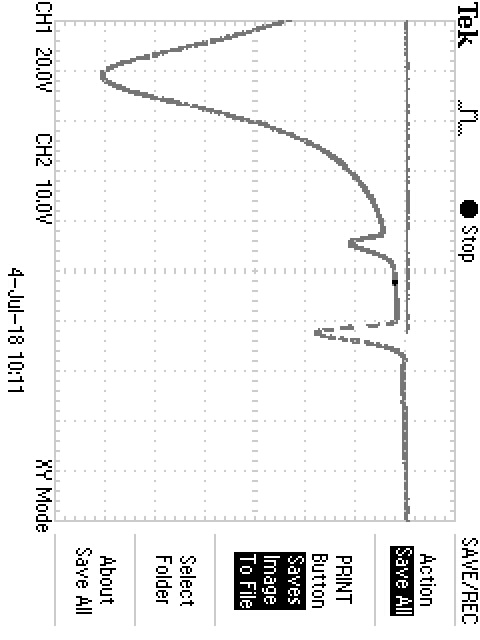
\includegraphics[angle = 90]{TEK0022.JPG}
  \caption{Bild einer Resonanzkurve auf einem Oszilloskop. Zu sehen sind, von Links nach Rechts, das Transparenzminimum bei 0, sowie die Resonanzen der beiden Rubidiumisotope A und B}
  \label{fig:Ausdruck}
\end{figure}
\begin{table}[H]
  \centering
  \caption{Messdaten aus der Vermessung der Minima und daraus berechnete Anteile.}
  \label{tab:Anteil}
  \begin{tabular}{c|c|c}
    &Isotop A & Isotop B\\
    \hline
    Tiefe in cm& 1.35& 2.1\\
    Anteil in \%&38.84&60.86\\
    Literaturwert:&27.83&72.17\\
    Abweichung in \%&39.56&15.67\\
  \end{tabular}
\end{table}

\subsection{Abschätzung des quadratischen Zeeman-Effekts}
Die Abstände zwischen den Zeeman-Niveaus ergeben sich bei genauerer Betrachtung aus einer Entwicklung der Energie in einer Potenzreihe gemäß
\begin{equation}
  U_{HF} = g_F \mu_B B + g_{f}^2 B^2 \mu_0^2 \frac{(1-2 M_F)}{\Delta E_{Hy}} - ...
  \label{eqn:potenz}
\end{equation}
Betrachtet man den linearen und quadratischen Term dieser Gleichung einzeln, so kann eine Abschätzung für den quadratischen Zeeman Effekt gegeben werden. Dazu werden aus den Messwerten für jede Messung eine obere (1000 Hz) Grenze für das Magnetfeld als Abschätzung verwendet. In Tabelle \ref{tab:quad} sind diese Werte dargestellt.
Die Abstände der Niveaus der Hyperfeinstruktur aufspaltung werden der Anleitung\cite{Anleitung} entnommen und Lauten $\Delta E_{hy} = 4.53\cdot 10^{-24}\si{\joule}$ für $\symup{^{85}Rb}$ und $\Delta E_{hy} = 2.01\cdot 10^{-24}\si{\joule}$ für $\symup{^{87}Rb}$.
Außerdem werden die magnetischen Quantenzahlen $\symup{M_F} = 3$ für $\symup{^{85}Rb}$ und $\symup{M_F} = 2$ für $\symup{^{87}Rb}$. Diese Werte ergeben sich aus dem Kernspin und dem Spin der Elektronenhüllen.\\
\begin{table}[H]
  \centering
  \caption{Gegenüberstellung des linearen und quadratischen Zeeman-Effektes für beide Messungen. Es sind jeweils die unteren und oberen Abschätzungen für beide Isotope angegeben. Die Werte für das Magnetfeld wurden Tabelle \ref{tab:gesamt1} und \ref{tab:gesamt2} entnommen.}
  \label{tab:quad}
  \begin{tabular}{c|cc}
    Messung 1:& Isotop A & Isotop B\\
    \hline
    linear oben & $(4.65 \pm 0.12)\cdot 10^{-28}\si{\joule}$ & $(4.51 \pm 0.08)\cdot 10^{-28}\si{\joule}$\\
    quadratisch oben & $(1.43 \pm 0.08)\cdot 10^{-31}\si{\joule}$ & $(5.07 \pm 0.18)\cdot 10^{-31}\si{\joule}$\\
    \hline
    Messung 2: &&\\
    \hline
    linear oben & $(4.73 \pm 0.08)\cdot 10^{-28}\si{\joule}$ & $(4.53 \pm 0.15)\cdot 10^{-28}\si{\joule}$\\
    quadratisch oben & $(1.48 \pm 0.16)\cdot 10^{-31}\si{\joule}$ & $(5.10 \pm 0.34)\cdot 10^{-31}\si{\joule}$\\
    \hline
  \end{tabular}
\end{table}
Anhand der Tabelle \ref{tab:quad} erkennt man, dass die Abschätzungen des quadratischen Zeeman-Effekts um minimal 5 Größenordnungen kleiner als die des linearen Zeeman-Effekts sind.
